 \let\negmedspace\undefined
\let\negthickspace\undefined
\documentclass[journal]{IEEEtran}
\usepackage[a5paper, margin=10mm, onecolumn]{geometry}
%\usepackage{lmodern} % Ensure lmodern is loaded for pdflatex
\usepackage{tfrupee} % Include tfrupee package

\setlength{\headheight}{1cm} % Set the height of the header box
\setlength{\headsep}{0mm}     % Set the distance between the header box and the top of the text
\usepackage{gvv-book}
\usepackage{gvv}
\usepackage{cite}
\usepackage{amsmath,amssymb,amsfonts,amsthm}
\usepackage{algorithmic}
\usepackage{graphicx}
\usepackage{textcomp}
\usepackage{xcolor}
\usepackage{txfonts}
\usepackage{listings}
\usepackage{enumitem}
\usepackage{mathtools}
\usepackage{gensymb}
\usepackage{comment}
\usepackage[breaklinks=true]{hyperref}
\usepackage{tkz-euclide} 
\usepackage{listings}
% \usepackage{gvv}                                        
\def\inputGnumericTable{}                                 
\usepackage[latin1]{inputenc}                                
\usepackage{color}                                            
\usepackage{array}                                            
\usepackage{longtable}                                       
\usepackage{calc}                                             
\usepackage{multirow}                                         
\usepackage{hhline}                                           
\usepackage{ifthen}                                           
\usepackage{lscape}



\usepackage{amsmath,amssymb}
\usepackage{booktabs}
\usepackage{tikz}
\usetikzlibrary{arrows.meta,angles,quotes}





\begin{document}

\bibliographystyle{IEEEtran}
\vspace{3cm}

\title{4.12.26}
\author{AI25BTECH11021 - Abhiram Reddy N}
% \maketitle
% \newpage
% \bigskip
{\let\newpage\relax\maketitle}

\renewcommand{\thefigure}{\theenumi}
\renewcommand{\thetable}{\theenumi}
\setlength{\intextsep}{10pt} % Space between text and floats


\numberwithin{equation}{enumi}
\numberwithin{figure}{enumi}
\renewcommand{\thetable}{\theenumi}


\section*{Question}

Prove that the locus of the foot of the perpendicular from the origin $O$ on the line $\frac{x}{a} + \frac{y}{b} = 1$, which satisfies the condition $\frac{1}{a^2} + \frac{1}{b^2} = \frac{1}{c^2}$ (where $c$ is a constant), is given by the circle $x^2 + y^2 = c^2$, using vector algebra with matrix notation and transpose.


\section*{Steps to Solve}

\subsection*{1. Vector and Matrix Representation of the Line and Points}

The equation of the line $L$ in intercept form is:
$$\frac{x}{a} + \frac{y}{b} = 1$$
We can express the line's equation in the form $\mathbf{r}^T \mathbf{n} = 1$, where $\mathbf{r} = \begin{pmatrix} x \\ y \end{pmatrix}$ and $\mathbf{n} = \begin{pmatrix} 1/a \\ 1/b \end{pmatrix}$:
$$L: \begin{pmatrix} x \\ y \end{pmatrix}^T \begin{pmatrix} 1/a \\ 1/b \end{pmatrix} = 1 \quad \text{(Equation 1)}$$

Let $P(x_0, y_0)$ be the foot of the perpendicular from the origin $O(0, 0)$. The position vector of $P$ is $\mathbf{p}$:
$$\mathbf{p} = \begin{pmatrix} x_0 \\ y_0 \end{pmatrix} \quad \text{(Equation 2)}$$



\subsection*{2. Condition of Perpendicularity and Point on the Line}

$\mathbf{OP}$ is Parallel to the Normal $\mathbf{n}$
The vector $\mathbf{p}$ (which is $\mathbf{OP}$) is perpendicular to the line $L$, hence it must be parallel to the line's normal vector $\mathbf{n}$:
$$\mathbf{p} = \lambda \mathbf{n} \quad \text{for some scalar } \lambda \quad \text{(Equation 3)}$$
$$\begin{pmatrix} x_0 \\ y_0 \end{pmatrix} = \lambda \begin{pmatrix} 1/a \\ 1/b \end{pmatrix} \implies x_0 = \frac{\lambda}{a}, \quad y_0 = \frac{\lambda}{b}$$
From these, we isolate the components of the normal vector:
$$\frac{1}{a} = \frac{x_0}{\lambda} \quad \text{and} \quad \frac{1}{b} = \frac{y_0}{\lambda} \quad \text{(Equation 4)}$$

$P$ lies on $L$
Since $P$ is on the line $L$, it must satisfy the line's equation (Equation 1):
$$\mathbf{p}^T \mathbf{n} = 1 \quad \text{(Equation 5)}$$
Substituting the scalar components:
$$\frac{x_0}{a} + \frac{y_0}{b} = 1$$
Now, substitute the expressions for $\frac{1}{a}$ and $\frac{1}{b}$ from (Equation 4):
$$x_0 \left(\frac{x_0}{\lambda}\right) + y_0 \left(\frac{y_0}{\lambda}\right) = 1$$
$$\frac{x_0^2 + y_0^2}{\lambda} = 1$$
$$x_0^2 + y_0^2 = \lambda \quad \text{(Equation 6)}$$
In matrix notation, the square of the distance from the origin to $P$ is:
$$\mathbf{p}^T \mathbf{p} = \lambda \quad \text{(Equation 7)}$$



\subsection*{3. Using the Given Locus Condition}

The line satisfies the condition:
$$\frac{1}{a^2} + \frac{1}{b^2} = \frac{1}{c^2} \quad \text{(Equation 8)}$$

Substitute the expressions for $\frac{1}{a}$ and $\frac{1}{b}$ from (Equation 4) into (Equation 8):
$$\left(\frac{x_0}{\lambda}\right)^2 + \left(\frac{y_0}{\lambda}\right)^2 = \frac{1}{c^2}$$
$$\frac{x_0^2 + y_0^2}{\lambda^2} = \frac{1}{c^2} \quad \text{(Equation 9)}$$

Now, substitute $x_0^2 + y_0^2 = \lambda$ (from Equation 6) into (Equation 9):
$$\frac{\lambda}{\lambda^2} = \frac{1}{c^2}$$
$$\frac{1}{\lambda} = \frac{1}{c^2} \implies \lambda = c^2 \quad \text{(Equation 10)}$$



\subsection*{4. Final Locus Equation}

Substitute $\lambda = c^2$ (Equation 10) back into the expression for $P$'s coordinates (Equation 6) or (Equation 7):
$$x_0^2 + y_0^2 = c^2$$
$$\mathbf{p}^T \mathbf{p} = c^2 \quad \text{(Equation 11)}$$

The locus of the foot of the perpendicular $P(x_0, y_0)$ is therefore:
$$x^2 + y^2 = c^2 \quad \text{(Equation 12)}$$
This is the equation of a circle centered at the origin with radius $c$.



\begin{figure}[htbp]
\centering
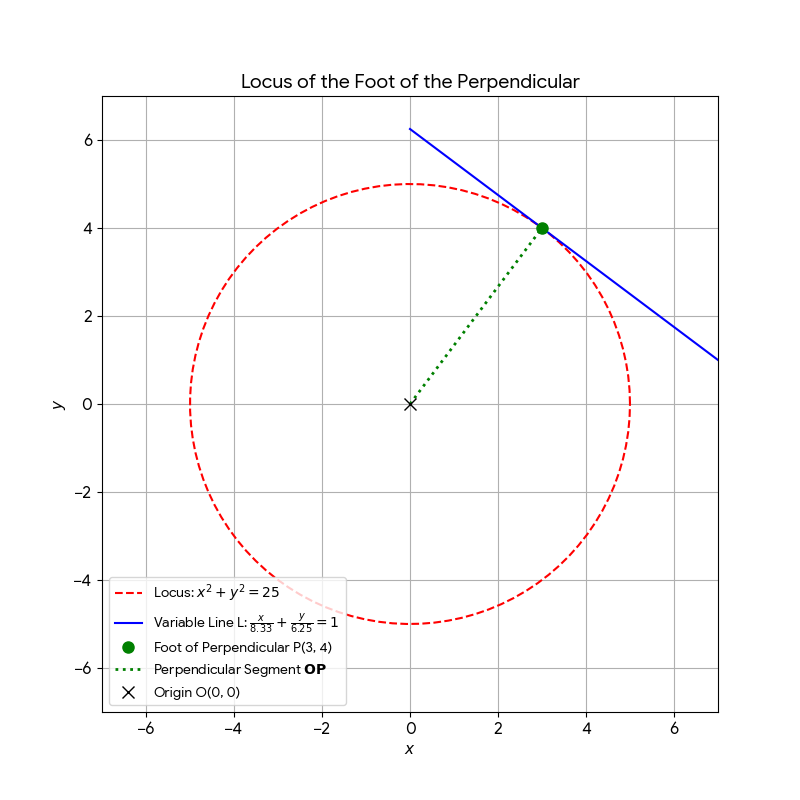
\includegraphics[width=\columnwidth]{figs/python_plot.png} 
\caption*{Plot of the curves}
\label*{Fig1}
\end{figure}


\end{document}

